\chapter{Introducción específica} % Main chapter title

\label{Chapter2}

%----------------------------------------------------------------------------------------
Este capitulo expone una descripción detallada del sistema, del hardware utilizado y las herramientas de  software necesarias en el desarrollo del trabajo. Se abarcan la descripcion del sistema y sus componentes, los \textit{frameworks} y modelos utilizados para detección facial y las herramientas utilziadas en la web.

%----------------------------------------------------------------------------------------
\section{Diagrama general del sistema}
El sistema desarrollado en este trabajo consta de varios componentes de hardware que interconectados entre si son capaces de cubrir . En la figura \ref{fig:sys_blocks} se muestra el diagrama en bloques del sistema.

\begin{figure}[h]
	\centering
	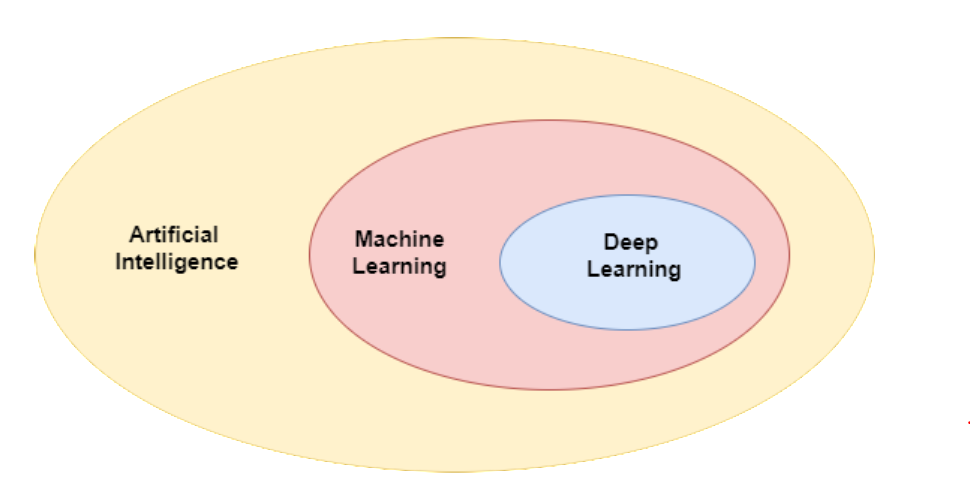
\includegraphics[scale=0.3]{./Figures/ai_ml_dl.png}
	\caption{Diagrama en bloques del sistema.}
	\label{fig:sys_blocks}
\end{figure}

\subsection{Placa de desarrollo ESP32-S3-DevKitC-1}
El componente central del sistema es la tarjeta de desarrollo ESP32-S3-DevKitC-1-N8R8 de la empresa Espressif. Tiene como componente central el modulo ESP32-S3-WROOM-1-N8R8 y varios otros componentes que simplifican el proceso de desarollo de aplicaiones para IoT. En la figura \ref{fig:devkit_comp} se observa una fotografia de la tarjeta con el detalle de sus componentes.

\begin{figure}[h]
	\centering
	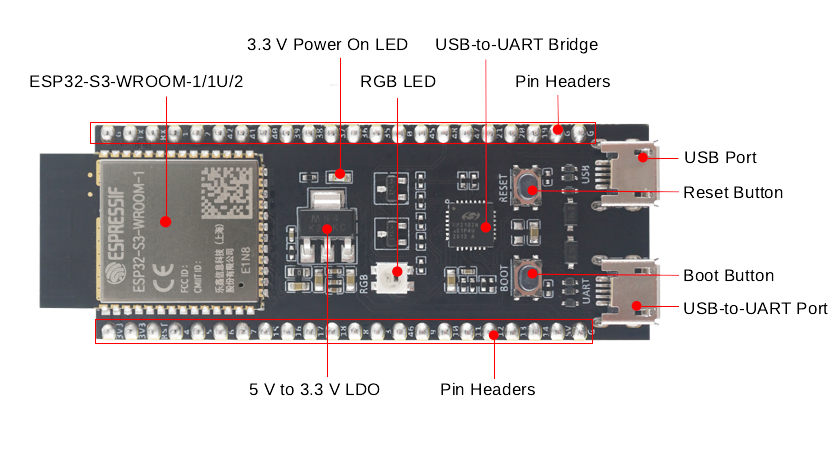
\includegraphics[scale=0.4]{./Figures/devkit_comp.png}
	\caption{Componentes del ESP32-S3-DevKitC-1.}
	\label{fig:devkit_comp}
\end{figure}

El modulo ç-WROOM-1-N8R8 es un potente modulo MCU (\textit{Microcontroller Unit}, Unidad de Microcontrolador) de doble nucleo que incorpora Wi-Fi y BLE (\textit{Bluetooth Low Energy}, Bluetooth de Baja Energia) y tiene un amplio conjunto de perifericos. Sus especificaciones tecnicas mas relevante son:
\begin{itemize}
	\item SoC embebido: ESP32-S3R8
	\item Procesador: Xtensa LX7 doble nucleo de 32 bits hasta 240 Mhz
	\item ROM: 384 KB
	\item SRAM: 512 KB
	\item Pines: 41
	\item Flash: 8 MB
	\item PSRAM (\textit{Pseudostatuc RAM}, RAM Pseudiestatica): 8 MB
	\item Tipo de antena: PCB
	\item Wi-Fi: 802.11 b/g/n hasta 150 Mbps
	\item Bluetooth: Bluetooth 5 y Bluetooth \textit{mesh}
	\item Perifericos: GPIO, I2C, SPI, interfaz LCD, interfaz de camara, UART, I2S, USB, PWM, ADC, sensor tactil, sensor de temperatura, timer y \textit{watchdogs}
	\item Temeperatura:  –40 ~ 65 °C
\end{itemize}

En el mercado existen muchos fabricantes que ofrecen tarjetas de desarrollo de caracteristicas tecnicas que podrian haber sido utilizadas para el desarrollo de este trabajo. Sin ir muy lejos, Espressif, fabricante de la ESP32-S3-DevKitC-1-N8R8, tiene toda una familia de modulos y tarjetas muy similares entre si. La eleccion de esta tarjeta en particular responde a los siguientes criterios:
\begin{itemize}
	\item Costo: Espressif ofrece en todos sus SoCs, modulos y tarjetas, un costo muy contenido por la gran cantidad de caracteristicas ofrecidas.
	\item Redes neuronales: la serie de SoCs ESP32-S3 ofrece soporte para instrucciones vectoriales, que acelera las tareas de computacion de redes neuronales. Esta fue la caracteristica mas importante al momento de la eleccion de esta tarjeta.
	\item Memoria: como el trabajo implicaba el uso de una camara y por tanto el manejo de \textit{buffers} de memoria de gran tamano para manipular las imagenes obtenidas, la cantidad de memoria externa que ofrecia esta tarjeta la hizo optima para la aplicacion. 
\end{itemize}

\subsection{Sensor de movimiento PIR}
Un sensor de movimiento PIR basa su funcionamiento al detectar diferencias en la energia IR (\textit{Infrared}, Infrarojo) en el campo de vision del sensor. Debido a que la senal de salida generada por el sensor es muy pequena, es necesario aplicar etapas de amplificacion y filtrado para elevar el nivel de tension de la senal de salida y al mismo tiempo filtrar el ruido que puede generar eventos falsos positivos. Esta salida analogica luego se debe convertir en una senal digital mediante la operacion de comparacion de ventanas y se puede utilizar, por ejemplo, como una interrupcion en un MCU. En la figura \ref{fig:move_blocks} se muestra el diagrama en bloques del sensor de movimiento PIR.

\begin{figure}[h]
	\centering
	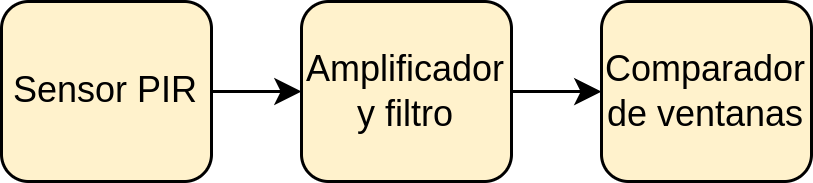
\includegraphics[scale=0.4]{./Figures/move_blocks.png}
	\caption{Diagrama en bloques del sensor de movimiento PIR.}
	\label{fig:move_blocks}
\end{figure}

\subsubsection{Sensor IRA-S230ST01}


\subsubsection{Amplificador operacional TVL8544}

\subsection{Cámara OV2640}
Otro de los componentes principales del sistema es la camara, que permite obtener imagenes en un formato digital que posteriormente deben ser procesadas por los algoritmos de DL. Para este trabajo se utilizo el modulo ESP-LyraP-CAM. Este modulo integra un CCM (\textit{Compact Camera Module}, Modulo de Camara Compacto) con un sensor OV2640 en conjunto con dos reguladores de tension para su correcto funcionamiento. En la figura \ref{fig:camera_blocks} se puede observar unas fotografias del modulo ESP-LyraP-CAM y sus componentes.

\begin{figure}[h]
	\centering
	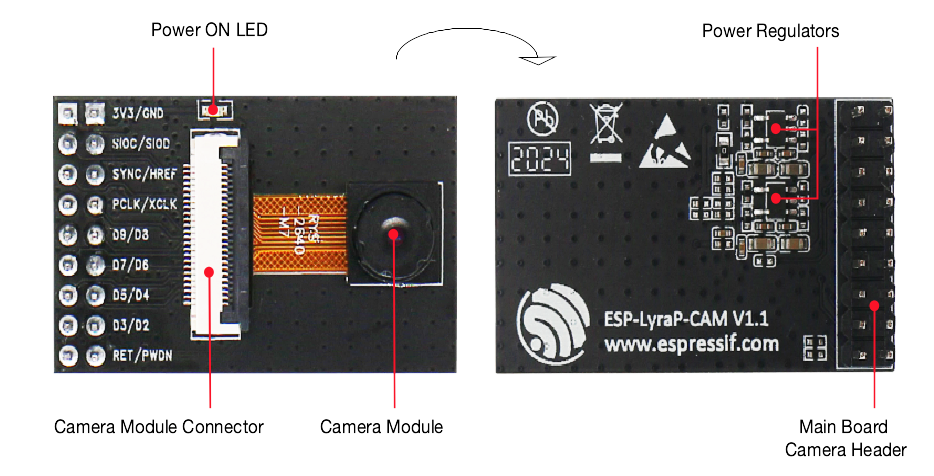
\includegraphics[scale=0.5]{./Figures/camera_blocks.png}
	\caption{Diagrama en bloques del del modulo ESP-LyraP-CAM.}
	\label{fig:camera_blocks}
\end{figure}

El OV2640 de la empresa OmniVision es un sensor CMOS (\textit{Complementary Metal-Oxide-Semiconductor}, Semiconductor de Oxido de Metal Complementario) de 2 MP, cuenta con una interfaz de comunicacion compatible con DVP  (\textit{Digital Video Port}, Puerto de Video Digital), soporta codificacion JPEG (\textit{Joint Photographic Experts Group}, Grupo Unido de Expertos en Fotografia) y es de bajo consumo energetico. En la tabla \ref{tab:ov2640_specs} se muestran las caracterisiticas tecnicas mas importantes del OV2640.

 \begin{table}[h]
	\centering
	\caption[OV2640 especificaciones]{Tabla de especificaciones del OV2640}
	\begin{tabular}{lc}    
		\toprule
		\textbf{Caracteristica} 	 & \textbf{Descripcion}  \\
		\midrule
		Tamano de matriz & 1600x1200 (UXGA) \\		
		Fuente de alimentacion & \begin{tabular}{@{}c@{}} \textit{Core}: 1.3 V ± 5\% \\ \textit{Analog} 2.5 ~ 3.0 V \\ I/O: 1.7 V - 3.3 V\end{tabular} \\
		Consumo energetico & \begin{tabular}{@{}c@{}} \textit{Free running}: 125 mW \\ \textit{Standby}: 600 \textmu A \end{tabular} \\
		Formato de imagen del sensor & 1/4'' \\
		Tasa de transferencia maxima & \begin{tabular}{@{}c@{}} 1600×1200 a 15 fps \\ SVGA a 30 fps \\ CIF a 60 fps \end{tabular} \\
		Sensibilidad & 0.6 / Lux-sec \\
		SNR & 40 dB \\
		Rango dinamico & 50 dB \\
		Tamano de pixel & 2.2x2.2 \textmu m \\
		Formato de salida & YUV/RGB/MJPEG \\
		\bottomrule
		\hline
	\end{tabular}
	\label{tab:ov2640_specs}
\end{table}

Los criterios para utilizar este modulo como camara del sistema son los siguientes:
\begin{itemize}
	\item Costo: los modulos con el sensor OV2640 tienen un costo muy reducido en comparacion con otros disponibles en el mercado.
	\item Bajo consumo energetico: como se mostro en la tabal \ref{tab:ov2640_specs} el consumo energetico del modulo en modo \textit{standby} es lo suficientemente bajo como para funcionar alimentado por baterias.
	\item Disponibilidad de codigo: al ser un modulo que ya lleva mucho tiempo en el mercado existen muchas bibliotecas de codigo para utilizarlo, lo que simplifica en gran medida el tiempo de desarrollo de \textit{firmware}.
\end{itemize}

%----------------------------------------------------------------------------------------
\section{MTCNN (\textit{Multi-Task Cascaded Convolutional Networks}, Redes Convolucionales en Cascada Multitarea)}

%----------------------------------------------------------------------------------------
\section{TensorFlow}

%----------------------------------------------------------------------------------------
\section{AWS (\textit{Amazon Web Services}, Servicios Web de Amazon)}

%----------------------------------------------------------------------------------------
\section{Grafana}
